% !TeX spellcheck = es
\documentclass[11pt, titlepage]{article}

\usepackage[spanish,mexico]{babel}
\usepackage{xcolor}
\definecolor{darkblue}{rgb}{0.1 , 0.1, 0.7}
% hyperrefs antes de geometry!
\usepackage[
hyperfootnotes=true,
urlcolor=blue,
colorlinks=true,
linkcolor=darkblue,
citecolor=darkblue]{hyperref}

% Math text
%\usepackage[utf8]{inputenc}
\usepackage[a4paper,top=2cm,bottom=2cm,left=2cm,right=3cm,marginparwidth=1.75cm,headheight=28pt]{geometry}
%\usepackage[spanish, mexico]{babel}
\usepackage{graphicx}

%\usepackage[utopia]{mathdesign}
%\usepackage[T1]{fontenc}					% Output font encoding for international characters
%\usepackage[utf8]{inputenc}			% Encoding of files: utf8
%\renewcommand*\familydefault{\sfdefault} 	% Sans Serif as default font


\usepackage{amsmath,array,IEEEtrantools,bm}
\usepackage{pdfpages}
% HEADER
\usepackage{fancyhdr,framed}
\setlength{\headheight}{44pt}
\pagestyle{fancy}
% TODO
\usepackage[
textwidth=2.6cm,
textsize=footnotesize,
]{todonotes}

\usepackage{natbib}

% !TeX root = ../main.tex



%% ROCKET
\newcommand{\CG}{{\mathrm{CG}}}
\newcommand{\LCG}{L_\CG}
\def\equilibrium{\mathrm{eq}}


%% DIFFERENTIAL OPERATOR
\makeatletter
\providecommand*{\diff}%
{\@ifnextchar^{\DIfF}{\DIfF^{}}}
\def\DIfF^#1{%
	\mathop{\mathrm{\mathstrut d}}%
	\nolimits^{#1}\gobblespace}
\def\gobblespace{%
	\futurelet\diffarg\opspace}
\def\opspace{%
	\let\DiffSpace\!%
	\ifx\diffarg(%
	\let\DiffSpace\relax
	\else
	\ifx\diffarg[%
	\let\DiffSpace\relax
	\else
	\ifx\diffarg\{%
	\let\DiffSpace\relax
	\fi\fi\fi\DiffSpace}

%% CONTROL:
\newcommand{\dimfont}[1]{\ensuremath{#1}}
\newcommand{\Cme}[1]{\mathbf{#1}}
\newcommand{\Mme}[1]{\mathbf{#1}}
\newcommand{\Nme}[1]{\mathrm{#1}}
\newcommand{\Ts}{T_s}

\newcommand{\eye}{\Mme{I}}
%transpose
\def\dt{\Delta t}
\def\tp{\!^{\top}\!}
% Small
\def\MA{\Mme{A}}
\def\MB{\Mme{B}}
\def\MC{\Mme{C}}
\def\MD{\Mme{D}}
\def\ME{\Mme{E}}

\def\MQ{\Mme{Q}}
\def\MR{\Mme{R}}
\def\MK{\Mme{K}}
\def\MW{\Mme{W}}
\def\MX{\Mme{X}}
\def\MV{\Mme{V}}
\def\ctrb{\Mme{Y}}
\def\Mzero{\Mme{0}}
\def\obsv{\Mme{\mathcal{O}}}

\newcommand{\ts}[2]{\left. #1\right|_{ #2}}

\def\error{\varepsilon}
\def\Cx{\Cme{x}}
\def\Cf{\Cme{f}}
\def\Cy{\Cme{y}}
\def\Cu{\Cme{u}}
\def\Cn{\Cme{n}}
\def\Cd{\Cme{d}}
\def\Czero{\Cme{0}}
\def\Cv{\Cme{v}}
\def\Cz{\Cme{z}}
\def\Cw{\Cme{w}}

\def\Jcost{\Cme{\mathcal{J}}}
% RK4
\def\Ca{\Cme{a}}
\def\Cb{\Cme{b}}
\def\Cc{\Cme{c}}


\def\noise{{n}}
\def\disturb{{d}}
\newcommand{\di}{\ensuremath{\textrm{d}}}

\newcommand{\Matlab}{{\sc Matlab}}

\def\matdiv{\bm{\textbackslash}}

\newcommand{\spartial}[2]{\frac{\partial {#1}}{\partial {#2}}}
\newcommand{\dpartial}[2]{\frac{\partial^2 #1}{\partial #2 ^2}}

%# ROBUST
\def\lap{\mathcal{L}}
\newcommand\lapc[1]{\lap \left\{#1\right\}}
\newcommand\ilapc[1]{\lap^{-1} \left\{#1\right\}}
\def\xbar{\bar{x}}
\def\ubar{\bar{u}} 

\def\MP{\Mme{P}}
\def\ML{\Mme{L}}
\def\MT{\Mme{T}}
\def\MS{\Mme{S}}


\def\Cr{\Cme{r}}
\def\Cn{\Cme{n}}

\def\openloop{{\textrm{\tiny{LA}}}}
\def\closedloop{{ \textrm{\tiny{LC}}}}
\def\true{{ \textrm{\tiny{real}}}}

% RIGID BODY MECHANICS
\newcommand{\frm}[1]{\mathrm{#1}}  % Frame of reference
\newcommand{\ogn}[1]{\mathcal{#1}} % Frame origin / point of reference
\newcommand{\skw}[1]{\tilde{#1}}   % skew matrix notation
\newcommand{\uveci}{{\bm{\hat{\textnormal{\bfseries\i}}}}}
\newcommand{\uvecj}{{\bm{\hat{\textnormal{\bfseries\j}}}}}
\DeclareRobustCommand{\uvec}[1]{{% Unit length vector of arbitrary orientation
		\ifcsname uvec#1\endcsname
		\csname uvec#1\endcsname
		\else
		\bm{\hat{\mathbf{#1}}}%
		\fi
}}
\DeclareRobustCommand{\avec}[1]{{%
		\underline{#1} %		\bm{\mathbf{#1}}%
}}
\DeclareRobustCommand{\bvec}[1]{{% Orthogonal basis vector
%		\ifcsname bvec#1\endcsname
%		\csname bvec#1\endcsname
%		\else
		\bm{\hat{\mathbf{#1}}}%
%		\fi
}}
\def\tform{\mathbf{A}}
\newcommand{\transform}[1]{\tform^\frm{#1}}
\newcommand{\dottransform}[1]{\dot{\tform}^\frm{#1}}
\def\attitude{\mathbf{H}}
\newcommand{\inertia}[2]{J_{\ogn{#1}}^{\frm{#2}}}
\newcommand{\inertiarotor}[2]{\inertia{\!\mathrm{r}#1}{#2}}


\makeatletter
\newcommand*\bigcdot{\mathpalette\bigcdot@{.5}}
\newcommand*\bigcdot@[2]{\mathbin{\vcenter{\hbox{\scalebox{#2}{$\m@th#1\bullet$}}}}}
\makeatother

% THEOREMS/ EXERCISES
\usepackage{amsthm}
\theoremstyle{definition}
%\newtheorem{definition}{Definition}[chapter]
%\newtheorem{theorem}{Teorema}[chapter]
%\newtheorem{exercise}{Ejercicio}[chapter]
\input{tex/code.tex}
% % !TeX root = ../pf-cretton-whitti.tex
\usepackage{amssymb}
\usepackage{alphalph}

\makeatletter
\newcommand*{\myfnsymbolsingle}[1]{%
	\ensuremath{%
 		\ifcase#1% 0
 		\or % 1
 		*%   
 		\or % 2
 		\dagger
 		\or % 3  
 		\ddagger
 		\or % 4   
 		\mathsection
 		\or % 5
 		\mathparagraph
 		\or
 		\lozenge
 		\or
 		\aleph
 		\or
 		\backepsilon
 		\or
 		\flat
 		\or 
 		\maltese
 		\or
 		\circledast
 		\or
 		\gimel
 		\or
 		\wp
 		\else % >= 7
 		\@ctrerr  
 		\fi
	}%   
}   
\makeatother

\newcommand*{\myfnsymbol}[1]{%
	\myfnsymbolsingle{\value{#1}}%
}

% remove upper boundary by multiplying the symbols if needed
\newalphalph{\myfnsymbolmult}[mult]{\myfnsymbolsingle}{}

\renewcommand*{\thefootnote}{%
	\myfnsymbolmult{\value{footnote}}%
}


\renewcommand*{\thefootnote}{%
	\myfnsymbolmult{\value{footnote}}%
}

\usepackage[sort=none,abbreviations]{glossaries-extra}
\setabbreviationstyle{long-short}

\newglossaryentry{corrutina}
{
	name=Corrutina,
    text=corrutina,
	description={Una unidad de procesamiento que puede ejecutarse en simultaneo con otras corrutinas.}
}

\newglossaryentry{esc}
{
	name=Electronic Speed Control,
	text=ESC,
	description={Controlador de velocidad para motores brushless. Suelen tener DC a la entrada y trifásica a la salida.}
}

\newglossaryentry{edf}
{
	name=Electronic ducted fan,
	text=EDF,
	description={Turbina impulsada por un motor eléctrico brushless. Es eficiente a altas velocidades.}
}

\newglossaryentry{lqr}
{
	name=Linear Quadratic Regulator,
	text=LQR,
	description={Regulador basado en control óptimo que busca reducir error cuadratico de una función costo.}
}

\newglossaryentry{soc}
{
	name=System on a chip,
	text=SoC,
	description={Integración de modulos conectados a un controlador en un único circuito impreso.}
}

\newglossaryentry{lia}
{
	name=LIA,
	text=LIA Aerospace,
	description={Laboratorio de Investigaciónes Aeroespaciales. Empresa para la cual se efectuó el desarrollo del vehículo.}
}

\newabbreviation{i2c}
{I$^2$C}
{Protocolo de comunicación de dos hilos que permite comunicar varios circuitos integrados en un bus.}

\newabbreviation{gpio}
{GPIO}
{Salida digital de uso genérico. Pueden estar en \emph{high} (tensión de fuente) o \emph{low} (puesto a tierra).}

\newabbreviation{spi}
{SPI}
{Serial peripheral interface. Un protocolo de comunicación full-duplex de Motorola.}

\newabbreviation{uart}
{UART}
{Protocolo de comunicación universal asincrono.}

\lhead{ LIA}
\newcommand{\mldivide}{\,{\boldsymbol{\backslash}}\,}
\usepackage{pdfpages}
\author{Patricio Whittingslow \and Luis Cretton}
\begin{document}
\begin{titlepage}
	
	\centering
	{\small LIA Aerospace \par}
	
	
	\vspace{8cm}
	{\Huge Gimballed EDF propelled VTVL vehicle design and control  \par}
	\vspace{2cm}
	{ \large {
			Patricio Whittingslow \\ Luis Cretton 
		\par}}
	\vspace{4cm}
	\today
	
\end{titlepage}

\begin{abstract}
En este documento se encuentran descriptas las secuencias del diseño, simulación, pruebas, y puesta en marcha de un vehículo autónomo VTVL (Vertical Take-off Vertical Landing). Se desarrolla la elección de un método de propulsión que lograra ensayar el sistema de control a baja escala para luego ser puesto en marcha en un sistema de mayor escala de uso sub-orbital o incluso orbital.


\end{abstract}

\newpage
\tableofcontents
\newpage
\printunsrtglossaries
\vfill
\hrule
\vspace{-1cm}
\subsection*{Nota del autor}
Si el documento es abierto desde un lector PDF moderno (Chrome, Adobe Acrobat Reader, entre otros), se podrá navegar el mismo mediante las referencias (haciendo click derecho).
\newpage

\section{Introducción}
El diseño, desarrollo, fabricación, armado, simulación y lanzamiento de cohetes, no es una tarea
sencilla ni repetida en intervalos de cortos de tiempo, al contrario, suelen llevar décadas y una
fuerte inversión para que sean posibles estos logros. El diseño y auge de vehículos VTVL viene
a subsanar estos factores ya que una vez terminada la misión el vehículo se puede reutilizar,
con mínimas intervenciones, y estaría listo para una nueva misión, atacando estos dos puntos principales anteriormente mencionados, el tiempo y el costo. Esto es a diferencia del método convencional donde el vehículo, luego de completar la misión, pasa a formar parte de basura espacial o, en el mejor de los casos, es recuperado del mar como el caso del Space Shuttle. 

\medskip

Los vehículos VTVL son tan viejos como el primer alunizaje. Traen en si varias ventajas frente a otros vehículos voladores como la gran reducción de espacio necesario para despegar y aterrizar. Esto no es un detalle menor dado que la mayor parte de la superficie terrestre de la tierra no son pistas de aterrizaje si no más bien terreno formado naturalmente.

\medskip

Este documento propone el diseño, simulación, control y fabricación de un vehículo con capacidades VTVL siendo un prototipo de baja escala. 
Este prototipo serviría como punta pie inicial
para vehículos de escala mayor que puedan completar misiones espaciales. Existen varias ventajas de implementar este tipo de tecnología.

\medskip

A baja escala, un vehículo que despega y aterriza por su cuenta, teniendo la capacidad de
superar obstáculos que se presenten, puede ser de gran utilidad en ambientes hostiles para el
ser humano, que esto se logre de manera rápida y efectiva podría ser la diferencia entre el
éxito o no de la misión.
Como ser el transporte de insumos médicos en tiempo real desde que un paciente lo requiere,
en zonas de acceso limitado.

\medskip

Últimamente hay un interés nuevo en imágenes espaciales. El vehículo podría ser utilizado para fines de sistemas de monitoreo y análisis geoespacial mediante el uso de estas imágenes, como hacen las empresas \textit{Ceres Imaging} y \textit{Satellogic}. %de una situación en la que no se disponga del tiempo suficiente para el accionar convencional a bajas velocidades como ser un helicóptero o un dron.  

\medskip

El vehículo una vez desarrollado y funcionando, puede servir de plataforma para diversos
estudios de fenómenos de dinámica de fluidos, como ser, mediciones aerodinámicas,
investigación del \textit{fuel sloshing} en vehículos con tanques esbeltos.

\medskip


Los sistemas de vehículos orbitales tienen sistemas complejos que deben ser testeados en una primera etapa mediante algún ensayo controlado. El vehículo que se desarrolla en el presente documento podría ser usado para tales fines como una plataforma para pruebas como ser el despliegue de una nariz o etapa, comprobación de sensores y actuadores a gran velocidad y con empuje variable.



\subsection{Estudio - Agua como propelente}
Se estudió la posibilidad de propulsar el vehículo con agua a presión. La figura \ref{fig:bottlerocket} muestra los resultados de una simulación de un vehículo pequeño de aluminio con un tanque a presión lleno en parte de agua y aire a 200 bar. En el mejor de los casos se llegaba a un tiempo de vuelo cercano a los 4 segundos que no es suficiente para comprobar un sistema de control. 

Para optimizar este problema se modificaba

\begin{itemize}
    \item Diámetro de la tobera -- más empuje vs. menos tiempo de vuelo controlado
    \item Volumen de agua -- más tiempo de vuelo vs. mayor peso de vehículo
\end{itemize}


\begin{figure}[htb]
    \centering
    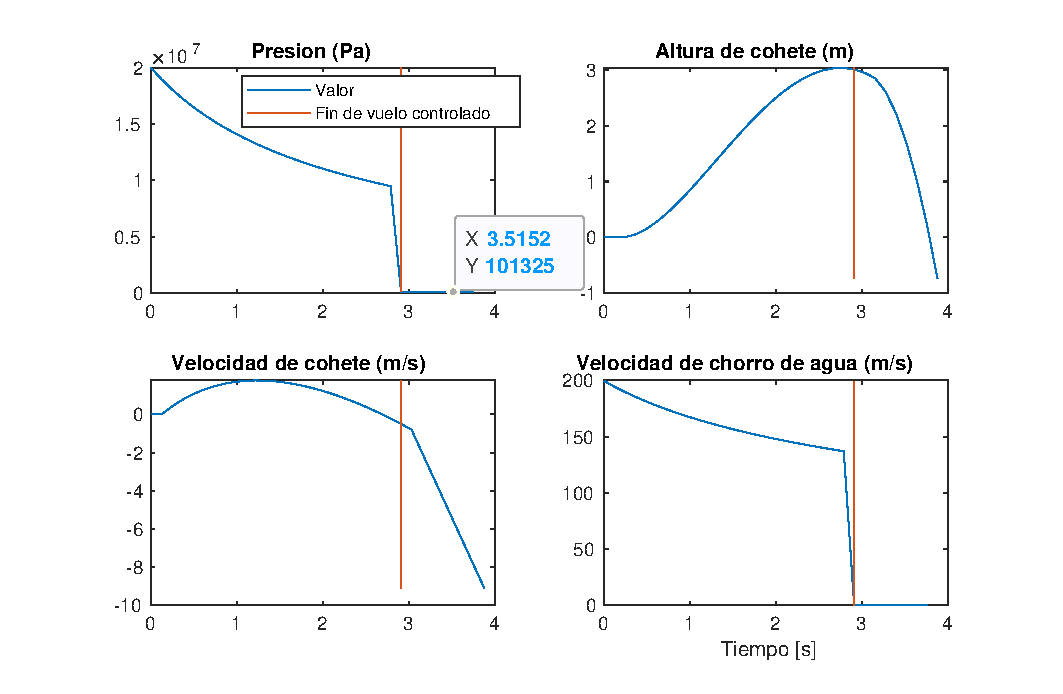
\includegraphics[width=0.8\linewidth]{fig/bottlerocket}
    \caption{Análisis preliminar para un vehículo propulsado por agua a presión. La presión es la del tanque (absoluta).}
    \label{fig:bottlerocket}
\end{figure}

\newpage


\subsection{Propulsión eléctrica}


\begin{figure}[htb]
    \centering
    \includegraphics[width=0.8\linewidth]{fig/vbat_icarus.png}
    \caption{Dos vehículos VTVL eléctricos modernos. ``VBat'' (Izq.) y ``Ikarus'' (Der.).}
    \label{fig:vbat_icarus}
\end{figure}

%Estos vehículos suelen ser la primera de muchas etapas para el desarrollo de un vehículo que cumple con los requisitos de la misión final.
Para lograr estas tareas generalmente los vehículos VTVL de baja escala generalmente son propulsados por motores eléctricos. %También existen alternativas al método de propulsión que se consideraron pero dado el alcance de un proyecto de universidad se decidió por un diseño compuesto por elementos comercialmente disponibles.\footnote{\textit{Commercial off the shelf} (COTS)}

\medskip

Los vehículos VTVL eléctricos son propulsados por hélices en su mayoría y constan casi siempre de 3 o más propulsores en un arreglo simétrico y plano. Recientemente hay un interés por la construcción de vehículos de una sola hélice por la buena relación empuje--peso que tienen. Sin embargo, estos vehículos no vienen sin sus complicaciones: 

\begin{itemize}
    \item La rotación dada al aire por la hélice causa un momento en el eje de propulsión que es contrarrestado en vehículos multirrotores.
    \item Inclinar al rotor durante su funcionamiento causa una fuerza perpendicular a la dirección de inclinación conocido como el efecto giroscópico. 
\end{itemize}

El primer punto es mitigado fácilmente agregando álabes a la salida del chorro para enderezar el flujo y contrarrestar la rotación. El segundo punto solo se resuelve conociendo las ecuaciones de momento angular y controlando actuadores con un sistema de control a lazo cerrado. Los sistemas vistos en la figura \ref{fig:vbat_icarus} tienen la particularidad de poder ser representados con relativa facilidad usando un solo marco de referencia inercial para el cálculo de las ecuaciones de momento angular. 

\section{Diseño}

En el marco de este proyecto, es de interés el diseño mecánico del mecanismo de control semejante un vehículo propulsado por combustión externa. Estos últimos suelen ser dirigidos por toberas montadas sobre un cardán. En el caso de un vehículo eléctrico de una hélice se tendría que montar el sistema de propulsión centrado en un gimbal para no obstruir el flujo.

\subsection{Selección de propulsador}

Existen diversas maneras de impulsar un vehículo de forma eléctrica. Luego de un cuidadoso estudio y discusión de ingeniería se decidió optar por un \gls{edf}, quien juega un rol central en el diseño pues es lo que se intenta controlar para llevar a cabo la navegación y guiado. Se analizo
ir por un EDF de aluminio, por una cuestión de durabilidad, relación empuje-peso, reducir probabilidad de fallas y roturas en sucesivos experimentos. 
Los EDF de aluminio solo se consiguen en el exterior y su precio es en dolares\footnote{El cambio de divisas es desfavorable para el lugar donde se desarrolla este proyecto.}. Esto trae varios inconvenientes en lo referente al presupuesto acotado, logística, compra y obtención. Los EDF
disponibles de plástico tienen una relación de empuje-diámetro mucho menor con respecto a
los de aluminio. Cabe destacar que el costo de un EDF de plástico y un EDF de aluminio son cercanos para diámetros similares.

\todo{Hablar del bucle}

\subsection{Diseño de la mecánica}

Para el diseño del gimbal se propuso una distribución de los mecanismos de actuación con
servos concéntricos a los ejes de rotación. Para evitar de esta manera complejidad de
mecanismos, cantidad de piezas de conexión entre servo y ejes, manufactura de mecanismos,
uniones rotoides, y obtener así un mapeo lineal del ángulo de actuación. El único intermediario
es el rodamiento que como se dispuso en la configuración ocupa el mínimo lugar posible justo
por encima de la estría del servo y se lleva las cargas.
Este mecanismo viene con la desventaja de una reducción de la resolución del ángulo de actuación comparado a un sistema actuado por un mecanismo biela-manivela.

\medskip

El material seleccionado para la fabricación del gimbal fue aluminio serie siete mil calidad
aeroespacial. Esta construido de una sola pieza, siendo el elemento que se lleva las tensiones
en todo momento en variabilidad de ángulos hacia el fuselaje, por ello la decisión de ser de la
serie de mayor resistencia mecánica de los aluminios comerciales.

\medskip

Los rodamientos seleccionados son de dimensiones 18mm exterior, 10mm interior y 7mm de espesor,
elegidos de esta manera por una cuestión de espacio para poder pasar la estría de los
servomotores por dentro, dejando un espesor de la pared del estriado de 2.5mm,
para evitar fisuras y hacer posible la manufactura de la pieza. La forma de generar el estriado
interno, es la de indentar con un patrón sobre un agujero previo de diámetro medio a los
valores máximos y mínimos de las crestas y valles de la estría. Esta operación debe hacerse con
el material en bruto para no arruinar las tolerancias que necesitan los rodamientos. Los
rodamientos se montarían clavados, minimizando el peso al no agregar seguers ni tapas con
bulones.

\medskip 

Los ejes del gimbal estarían en disposición simplemente apoyada y de forma axisimétrica para prevenir perturbaciones dinámicas por desbalanceo.

\medskip

Con respecto al fuselaje, al inicio se pensó una envolvente cilíndrica para el anillo externo del
gimbal. Luego se diseñó un desarrollo reticulado optimizado, se pasó por diferentes modelos e
ideas, hasta que se combinaron varios puntos fuertes de cada idea. La envolvente del gimbal se fabrica de forma rolada y optimizada en peso a raíz de
una planchuela de aluminio vaciada y luego generando su forma cilíndrica.\footnote{Contiene al
anillo del gimbal.} Esto distribuye las masas de manera más favorable con menos espacio
ocupado (dinámica-peso). Aguas arriba del gimbal se opto por un chasis tubular, con diversos
vaciados, que mediante flejes puede soportar cada elemento que se acopla al cohete por
medio de uniones abulonadas. Permitiendo mediante sus aberturas el acceso a cada
componente del vehículo, proporcionando, además, una renovación del aire para una
evacuación del calor generado, y un flujo abundante hacia la admisión del EDF.

\medskip

De la manera que se construye el gimbal puede entregar una rotación entera sin hacer contacto con la estructura. Se elige esta configuración por posibles desviaciones del proyecto en el
futuro, calculamos que utilizaremos menos de 20$^\circ$ de rotación de cada eje de gimbal ($\pm$10$^\circ$).

\subsection{Posición de baterías}

La la decisión de donde posicionar las baterías surgía de querer simular un vehículo semejante a los VTVL de la industria aeroespacial y también la posibilidad de tener una inercia favorable para los margenes de estabilidad. Estos dos últimos puntos sugieren que la posición ideal para las baterías es arriba de todo. Esto haría que el punto alrededor del cual se linealizó las ecuaciones de movimiento sea más estable. Luego de una conversación con Pablo Cossutta, un ingeniero electrónico especialista en sistemas de potencia, se optó por la configuración encontrada en el documento. Las baterías se encuentran cerca del EDF para alejar las líneas de potencia trifásica correspondientes al motor brushlesss de lo que es la electrónica digital. Al inestabilizar el punto de operación se obtiene una mejora en la respuesta ante actuaciones permitiendo una corrección de trayectoria más rápida.\footnote{Este resultado es deseado cuando se desea tener mejor rendimiento por ángulo de actuación, como sucede con los \textit{aviones caza} que utilizan este fenómeno a conveniencia.}


\subsection{Selección de servos} \label{ssec:servoSeleccion}
\newcommand{\micro}{\ensuremath{\mu}}
\newcommand{\grad}{\ensuremath{^\circ}}
Para obtener una buena respuesta del vehículo ante actuaciones se debe acotar la resolución necesaria. Según \cite{castillo2018efectos}, l aresolución angular de un servo es de 


\[
R_p = \frac{\theta \cdot T_D}{PW}  
\]
donde $\theta$ es el angulo de barrido del servo (especificado por el fabricante), $T_D$ es el tiempo muerto y $PW$ es el ancho de pulso operativo. 

El servo seleccionado es el SC1258TG. Tiene las siguientes especificaciones

\begin{itemize}
    \item Tiempo muerto (\textit{deadband}) 3\micro s
    \item Rango de ancho de pulso mínimo y máximo 800-2100\micro s
    \item Posición neutra 1500\micro s
    \item Ángulo de barrido operativo 100\grad (para 1000-2000\micro s)
    \item Velocidad 1,05 rad/s
\end{itemize}

Se tiene entonces una resolución mínima de 0,3\grad~ con un ancho de pulso de 2000\micro s. Esta resolución es alimentada como parámetro de actuación en las simulaciones.

\todo{Incluir estudio de resolución de servo}

\subsection{Contexto de pandemia}
Las medidas tomadas durante la pandemia por el gobierno fueron muy estrictas e influenció a todo tipo de acción que se quiso tomar. Durante el primer año de pandemia no nos pudimos reunir físicamente para discutir ideas de diseño, lo cual dificultó el avance físico del proyecto como así también la toma de decisiones y la comunicación entre partes, crucial en el inicio de todos proyectos de ingeniería.

\medskip

Una de las mayores complicaciones que se tuvo fue la compra de
componentes, además de la fabricación, que se vio afectada, por las políticas cambiantes de
nuestro país con respecto a la compra y la entrada de productos importados a suelo argentino.
Incluso la compra y llegada de los productos fue un motivo de festejo luego de un tortuoso
trayecto.





\section{Modelo 2D simplificado}

Esta siguiente sección detallará el tratamiento matemático efectuado para controlar un vehículo con propulsión vectorizada en el plano. El proposito es ilustrar a un nivel simple las herramientas que serán aplicadas para controlar el vehículo diseñado.

\begin{figure}[htb!]
	\centering
	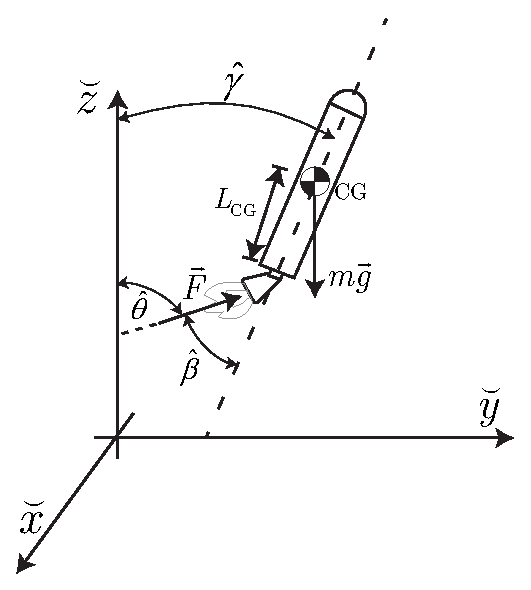
\includegraphics[width=9cm]{fig/rocketFBD.eps}
	\caption{Diagrama de cuerpo libre de un vehículo con propulsión vectorizada 2D.}
	\label{fig:FBD2D}
\end{figure}


\subsection{Modelado matemático}
Comenzamos con las ecuaciones dinámicas de un vehículo en el plano con control de propulsión vectorizada (por ángulo)

\[
\left\{
\begin{array}{l}
	\ddot{y}=\frac{F}{m} \sin(\gamma+\beta) \\
	\ddot{z}=\frac{F}{m} \cos (\gamma+\beta)-g \\
	\ddot{\gamma} = \frac{L_{\CG}\cdot F}{I_{xx}}\sin\beta
\end{array}
\right.
\]
donde \(\LCG\) y \(F\) están en función del tiempo, $m =m_0 - \int \dot{m} $ y $\theta = \gamma+\beta$. 

Vale la pena aclarar que no se tomarán en cuenta los siguientes efectos:
\begin{itemize}
	\item Fuerza de drag
	\item Viento
	\item \textit{Fuel sloshing}
	\item Efectos relativisticos
\end{itemize}

\subsection{Armado de sistema lineal}

Se propone un punto de operación alrededor del cual se linealizan las ecuaciones. El estado del vehículo es \textit{vertical y quieto en el espacio}. \footnote{La linealización esd valida solo para un vehículo vertical. Se debrá modificar el método para modelar un vehículo orbital.} 

\begin{align*}
	\gamma^* = 0 \\
	\beta^* = 0 \\
	F^* = mg
\end{align*}
en este caso $F$ es la desviación del punto de operación. Desde ahora en adelante $\Delta F = F- mg$.

\subsection{Representación en espacio de estados}
El número de variables de estado será igual a número de almacenadores de energía independientes. Estos son

\begin{enumerate}
	\item[$z$] Energía potencial por la gravedad
	\item[$\dot{y},\dot{z}$] Energía cinetica del vehículo
	\item[$\dot{\gamma}$] Momento angular del vehículo
\end{enumerate}
entonces, las variables de estado son las siguientes
\begin{align*}
	x_1 = y \\
	x_2 = \dot{y} \\
	x_3 = z \\
	x_4 = \dot{z} \\
	x_5 = \gamma \\
	x_6 = \dot{\gamma}
\end{align*}
donde $\dot{x_1} = x_2$, $\dot{x_3} = x_4$ y $\dot{x_5} = x_6$

Se aprovecha la expansión de Taylor para la linealización de expresiones trigonométricas:
\[
\sin(x+y)|_{x=x_0+\Delta x,y=y_0+\Delta y} \approx \sin(x_0+y_0) + \cos(x_0 + y_0) (x-x_0) + \cos(x_0 + y_0) (y-y_0)
\]

Las ecuaciones dinámicas de los estados 2,3, y 4 son dadas por las ecuaciones mostradas al comienzo de esta sección.
Abajo están las ecuaciones de estados
\begin{equation}
	\dot{x_2} = \frac{F}{m} \left( \gamma+\beta \right) = g x_5 + g u_2 
\end{equation}
\begin{equation}
\dot{x_4} = \frac{F}{m} - g =\frac{F-F_0}{m}= \frac{u_1}{m}
\end{equation}
\begin{equation}
\dot{x_6} = \frac{\LCG \cdot F}{I_{xx}} \beta = \frac{\LCG \cdot mg}{I_{xx}} u_2 
\end{equation}

donde $\Ts$ es el periodo de sampleo.

Los vectores de entrada y salida son
\[
\Cme{u}(t) = \begin{bmatrix}
u_1 \\
u_2
\end{bmatrix} = \begin{bmatrix}
\Delta F \\
\beta
\end{bmatrix}
\]
\[
\Cme{y}(t) = \begin{bmatrix}
y_1 \\
y_2 \\
y_3
\end{bmatrix} = \begin{bmatrix}
y \\
z \\
\gamma
\end{bmatrix}
\]
tal que las ecuaciones de salida son

\begin{equation}
	y_1 = x_1 
\end{equation}
\begin{equation}
	y_2 = x_3
\end{equation}
\begin{equation}
	y_3 = x_5
\end{equation}

Se escriben las matrices del sistema y de control ($\Mme{D} = [0]$)
\begin{equation} \label{eq:ssmatrices}
	\Mme{A} = 
	\left[\begin{array}{cccccc} 0 & 1 & 0 & 0 & 0 & 0\\ 0 & 0 & 0 & 0 & g & 0\\ 0 & 0 & 0 & 1 & 0 & 0\\ 0 & 0 & 0 & 0 & 0 & 0\\ 0 & 0 & 0 & 0 & 0 & 1\\ 0 & 0 & 0 & 0 & 0 & 0 \end{array}\right],\quad \Mme{B} = 
	\left[\begin{array}{cc} 0 & 0\\ 0 & g\\ 0 & 0\\ \frac{1}{m} & 0\\ 0 & 0\\ 0 & \frac{\LCG \cdot mg}{I_{xx}} \end{array}\right], \quad \Mme{C} =  \left[\begin{array}{cccccc} 1 & 0 & 0 & 0 & 0 & 0\\ 0 & 0 & 1 & 0 & 0 & 0\\ 0 & 0 & 0 & 0 & 1 & 0 \end{array}\right]
\end{equation}
El sistema mostrado en \eqref{eq:ssmatrices} es \textit{fully state controllable}.

\section{Ecuaciones de movimiento de cuerpo rígido} \label{sec:ecuacionesRigid}
A continuación se mostrarán las ecuaciones de movimiento en el espacio usadas para controlar el vehículo.
Se hará referencia a la figura \ref{fig:FBD2D} para explicar las variables en juego en el modelo 3D debido a la dificultad inherente de mostrar las 16 variables de estado en un dibujo del modelo 3D.

\begin{figure}[htb!]
	\centering
	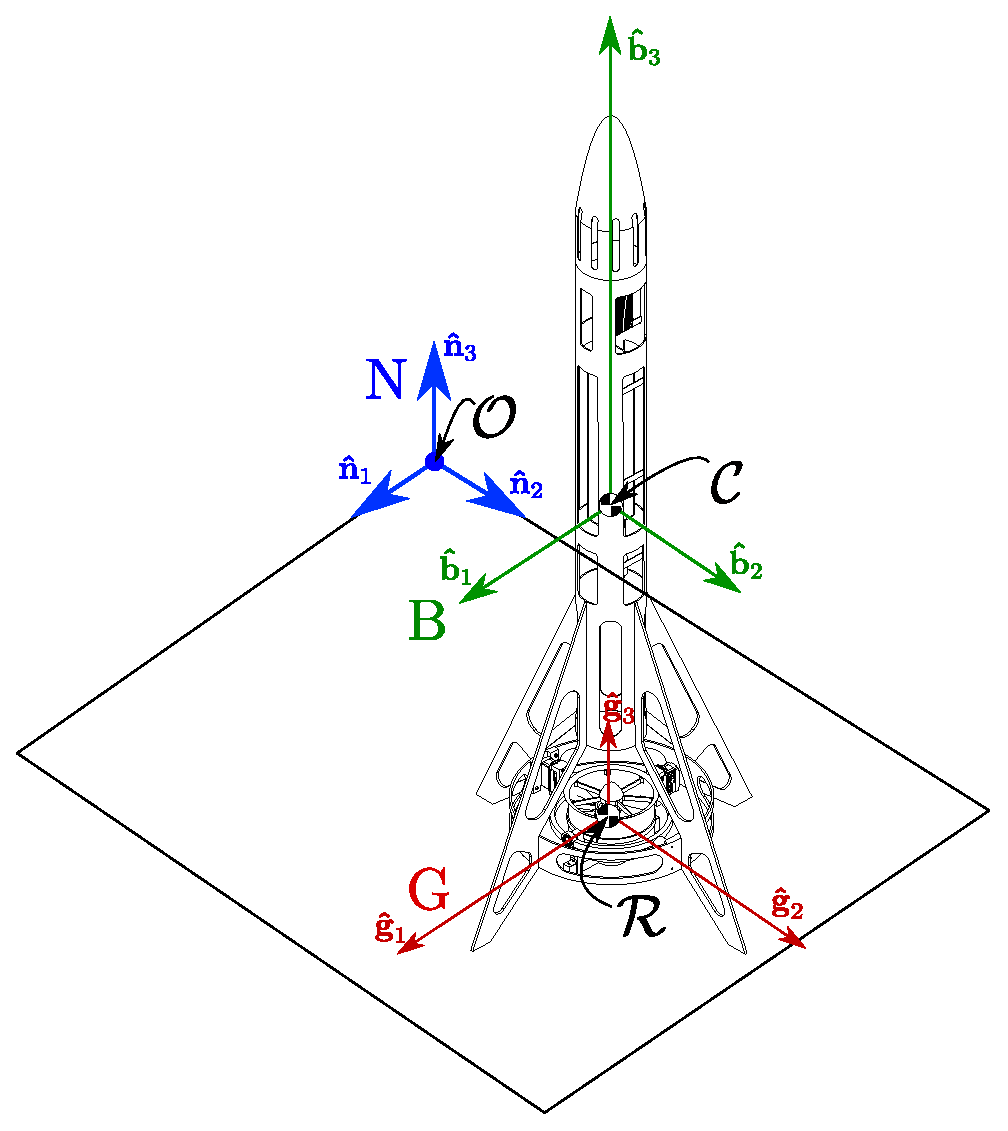
\includegraphics[width=0.52\textwidth]{fig/marcosDiagrama.eps}
	\caption{Marcos de referencia tomados para el análisis de cuerpo rígido. Por simplicidad se toman los centros de masa del cardán y del rotor como coincidentes en el punto $\ogn{R}$.}
\end{figure}

\newpage
\subsection{Notación}

La notación es la del libro \textit{Rigid Body Dynamics of Mechanisms, Theoretical Basics} \cite{hahn2013rigid}. Se requiere un tratamiento algebraico explicito de los marcos de referencia y representación debido al caso especial de un \textit{gimballed rotor}. Este tratamiento facilita la programación de la simulación y, en consecuencia, el control, el cual se volvería ambiguo y complejo con un tratamiento más común o simplificado.

\begin{description}
	\item[{\(\avec{r}_{\ogn{CO}}=[x,y,z]\)}] : Posición absoluta del centro de masa del vehículo léase ``posición de $\ogn{C}$ respecto $\ogn{O}$'')
	\item[{\(\avec{r}_{\ogn{RC}}\)}] : Posición del centro de masa del cardán respecto al centro de masa del vehículo
	\item[{\( \avec{\eta}=[\phi,\theta,\psi] \)}] : Ángulos de actitud del vehículo (Ángulos Euler)
	\item[\( \avec{\omega}_r^{\frm{G}} \)] : Velocidad angular del rotor del EDF representado en el marco $\frm{G}$ (dirección constante)
	\item[\( \avec{\omega}_\frm{BN}^\frm{B} \)] : Velocidad angular de $\frm{B}$ respecto a $\frm{N}$, representado en el marco $\frm{B}$.
	\item[\(  \alpha, \beta \)] : Ángulo de actuación de vectorización del EDF o ángulo de actitud del marco $\frm{G}$
	\item[{\( \delta   \)}] :  Ángulo de actuación de los dos flaps anti-roll
	\item[{\( m  \)}] :  Masa del vehículo sin rotor
	\item[{\( m_r  \)}] :  Masa del rotor
	\item[{\( \avec{g}  \)}] :  Aceleración de la gravedad
	\item[{\( \avec{F}^\frm{B} \)}] : Empuje del EDF representado en el marco $\frm{B}$ 
	\item[{\( \transform{NB}  \)}] :  Matriz de transformación de cosenos directores de un marco $\frm{B}$ a el marco $\frm{N}$
\end{description}

\textbf{Caracterización del EDF}
\begin{description}
	\item[{\( \tau_c  \)}] :  Torque efectivo de control del EDF
%	\item[{\( i  \)}] :  Corriente entregada al motor
	\item[{\( K_T  \)}] :  Constante de empuje del EDF
	\item[{\( K_Q  \)}] :  Coeficiente de torque viscoso de fricción
	\item[{\( Q  \)}] :  Torque viscoso de fricción
	\item[{\( \tau_r \)}] : Torque de reacción por el swirl de salida
\end{description}

\textbf{Caracterización del mecanismo anti-roll:}
\begin{description}
	\item[{\( K_{F_L}  \)}] : Coeficiente de lift de los flaps anti-roll
	\item[{\( K_{F_D}  \)}] : Coeficiente de drag de los flaps anti-roll
	\item[{\( F_L \)}] : Lift de los flaps anti-roll
	\item[{\( F_D \)}] : Drag de los flaps anti-roll
\end{description}

\textbf{Matriz de inercia:}
\begin{description}
	\item[{\(  \inertia{C}{B}  \)}] : Vehículo sin rotor respecto a $\ogn{C}$ representado en $\frm{B}$
	\item[{\(  \inertiarotor{R}{G}  \)}] : Rotor respecto a $\ogn{R}$ representado en $\frm{G}$
	\item[{\(  \inertia{\!\mathrm{g}R}{G}  \)}] : Cardán y motor sin rotor respecto a $\ogn{R}$ representado en $\frm{G}$
\end{description}



\subsection{Notación del álgebra a utilizar}

El producto escalar se define como $\bigcdot$ para diferenciarlo de simple multiplicación vectorial ($\cdot$). $\skw{\omega}$ es la matriz skew del vector que reemplaza el producto vectorial ya que $\skw{r}\cdot v = r \times v$
\[
\skw{\omega}_{L R}^{L}=\left(\begin{array}{ccc}
0 & -\omega_{z L R}^{L}, & \omega_{y L R}^{L} \\
\omega_{z L R}^{L} & 0 &-\omega_{x L R}^{L} \\
-\omega_{y L R}^{L} &  \omega_{x L R}^{L} & 0
\end{array}\right)
\]

Se dice que $J_\ogn{C}^\frm{B}$ es la matriz de inercia respecto el punto $\ogn{C}$, representado en el marco $\frm{B}$: es decir, las componentes de la matriz de inercia están en la base de $\frm{B}$. Esto se puede escribir así:
\begin{IEEEeqnarray*}{c}
J_\ogn{C}^\frm{B} = J_{b1} \bvec{b}_1 + J_{b2} \bvec{b}_2 + J_{b3} \bvec{b}_3
\end{IEEEeqnarray*}

La derivada del término anterior respecto un marco $N$ quedaría escrito
$${}^\frm{N}\dot{J}_{\ogn{C}}^\frm{B} =\left.^\frm{N} \frac{\di J_\ogn{C}^\frm{B}}{\di t}  \right. = \transform{NB} \cdot \left.^\frm{B} \frac{\di J_\ogn{C}^\frm{B}}{\di t}  \right. $$


Se pueden demostrar las siguientes ecuaciones
\begin{IEEEeqnarray}{C}
\dottransform{RL} =\transform{RL}\cdot \skw{\omega}^\frm{L}_\frm{LR} =
\skw{\omega}^\frm{R}_\frm{LR}\cdot\transform{LR} = -\skw{\omega}^\frm{L}_\frm{LR}\cdot\transform{RL} \\
\transform{BN} = (\transform{NB})\tp =  (\transform{NB})^{-1} \quad \Rightarrow \quad \transform{NB} \cdot \transform{BN} = \eye
\end{IEEEeqnarray}

donde $\omega_{\frm{LR}}^{\frm{L}}$ es la velocidad angular vectorial del marco $\frm{L}$ con respecto a $\frm{R}$ representado en $\frm{L}$, $\transform{RL}$ es la matriz de cosenos directores que transforma una vector de una base ortogonal $\frm{L}$ a otra base ortogonal $\frm{R}$, y $\dottransform{RL}$ es la derivada de la matriz $\transform{RL}$ respecto $\frm{R}$.

\newpage

\subsection{Variables de estado}
Se tendrán las variables de estado de posición y velocidad donde $z$ positivo es alejándose de la tierra.
\[
\avec{r}_\ogn{CO}^\frm{N} = 
\begin{bmatrix}
x & y & z 
\end{bmatrix}, \qquad
\dot{\avec{r}}_\ogn{CO}^\frm{N} = 
\begin{bmatrix}
\dot{x} & \dot{y} & \dot{z}
\end{bmatrix} 
\]

El movimiento cuerpo rígido será descrito por 3 ángulos de Euler (Cardán o Bryant en algunas bibliografías) $\phi, \theta$ y $\psi$ (roll, pitch, yaw respectivamente).
\begin{IEEEeqnarray}{C}
\avec{\eta} = \begin{bmatrix}
\phi  &  \theta &  \psi
\end{bmatrix}
\end{IEEEeqnarray}

\begin{figure}[ht!]
	\centering
	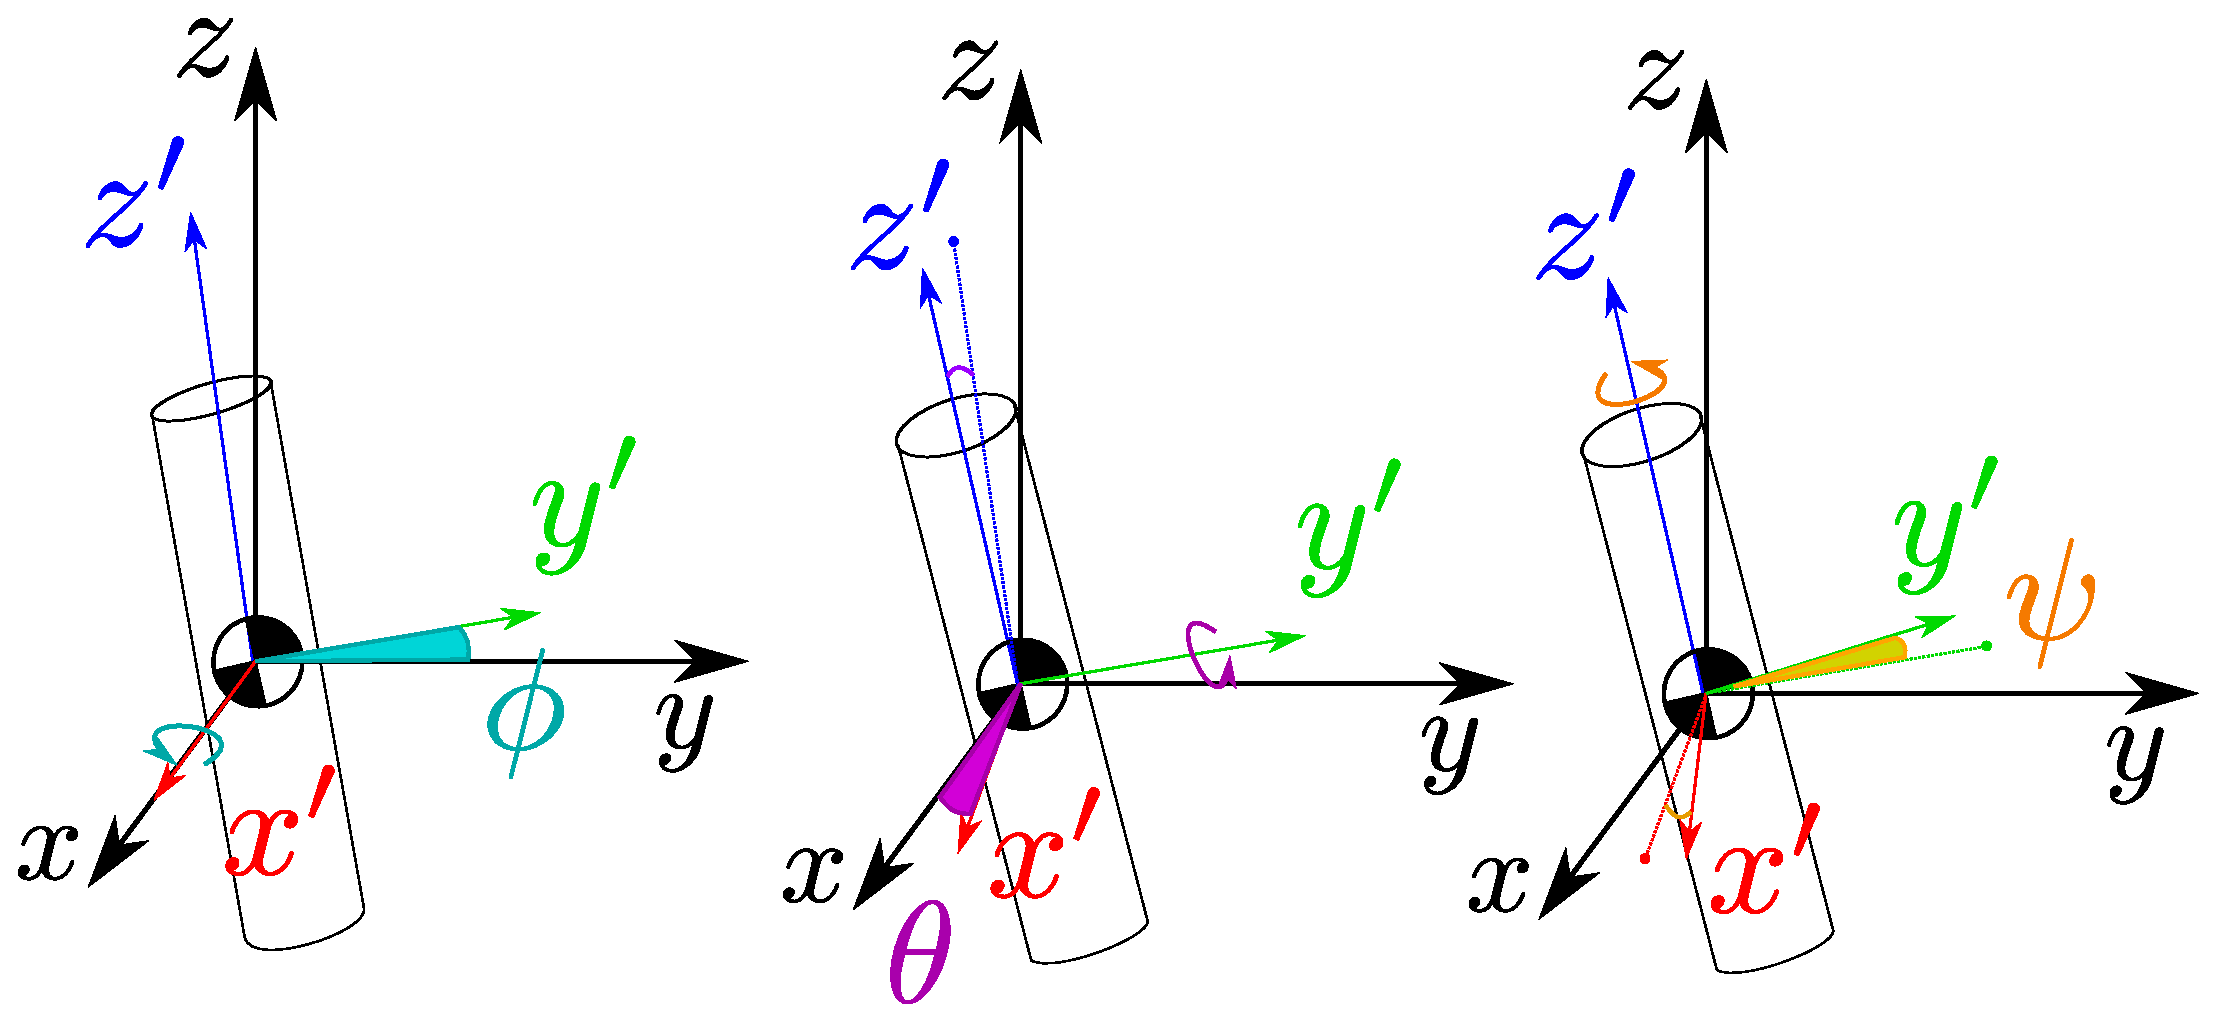
\includegraphics[width=0.8\textwidth]{fig/cuerpolibreGlobal_v2.eps}
	\caption{Diagrama mostrando las rotaciones de ángulo de euler en el orden que son efectuadas para describir el sistema. $\phi$ representa el pitch, $\theta$ el yaw y $\psi$ el roll. Se muestran las últimas posiciones de los ejes rotados con una linea punteada.}
\end{figure}


Los ángulos de la vectorización de la tobera serán $\alpha$ y $\beta$. $\delta$ corresponde a los actuadores que contrarrestan el roll del vehículo mediante dos flaps. Los ángulos $\alpha$ y $\beta$ describen la dirección en la que está apuntando la tobera (equivalente a la orientación $\frm{G}$) respecto la dirección del vehículo (marco $\frm{B}$). $\omega_r=\omega_r^\frm{G}$ es la velocidad angular del rotor.

\medskip

Se escriben las variables de estado y el vector input, donde $F$ es la fuerza que hace la tobera sobre el vehículo (la cual depende de la velocidad del vehículo)\footnote{En el código $\phi$, $\theta$ y $\psi$ aparecen como \texttt{q,r,s}}
\begin{equation} \label{eq:ssVariables3D}
	\Cx = \left[
	\begin{array}{cccccccc}
		\avec{r}_\ogn{CO}^\frm{N} & \avec{\eta} &\dot{\avec{r}}_\ogn{CO}^\frm{N} &  \avec{\omega}_\frm{BN}^\frm{B} & \omega_r & \alpha & \beta & \delta
	\end{array}\right] \tp
\end{equation}
\begin{equation}\label{eq:ssInputs3D}
	\Cu = \begin{bmatrix}
		\tau_c & \dot{\alpha} & \dot{\beta} & \dot{\delta}
	\end{bmatrix} \tp
\end{equation}
En la próxima sección se buscará obtener el vector de variables de estado derivado en el tiempo $\dot{\Cx}$.

\subsection{Ecuaciones diferenciales} \label{subsec:modeloMatematico}

\def\scos{\operatorname{c}}
\def\ssin{\operatorname{s}}
Definimos la transformación de los ángulos euler con una matriz de transformación $\transform{BN}$ donde $\scos$ y $\ssin$ son las funciones coseno y seno, respectivamente.

\begin{equation} \label{eq:matrizTransfoVehiculo}
	\transform{BN} = \begin{bmatrix}
	\scos \theta \cdot \scos \psi & \scos \theta \cdot \ssin \psi & - \ssin \theta \\
	\ssin \phi \cdot \ssin \theta \cdot \scos \psi - \scos \phi \cdot \ssin \psi & \ssin\phi \cdot \ssin\theta \cdot \ssin\psi + \scos\phi\cdot\scos\psi & \ssin\phi \cdot \scos\theta \\
	\scos\phi \cdot \ssin\theta \cdot \scos\psi + \ssin\phi \cdot \ssin\psi\quad & \scos\phi \cdot \ssin\theta \cdot \ssin\psi - \ssin\phi \cdot \scos\psi \quad& \scos\phi \cdot \scos\theta
	\end{bmatrix}
\end{equation}
La transformación nos servirá para poder pasar de la dinámica que está definida en el marco del vehículo $\frm{B}$ al marco $\frm{N}$ donde se tienen las variables de estado que se desean controlar.

Podemos obtener la velocidad en el marco del cuerpo
\begin{IEEEeqnarray}{rCl}
	\dot{\avec{r}}_\ogn{CO}^\frm{B} &= &\transform{BN} \cdot \dot{\avec{r}}_\ogn{CO}^\frm{N} 
\end{IEEEeqnarray}

La obtención de la velocidad angular del cuerpo se complica por el hecho que la razón de cambio de los ángulos de Euler no son vectores cartesianos, si no más bien parámetros que describen la orientación del cuerpo rígido en el espacio.\footnote{ Como bien sabemos la matriz de transformación $\tform$ solo es aplicable para transformar vectores cartesianos de una base ortogonal a otra. Los parámetros $\avec{\eta}$ conforman un vector de configuración, no un vector cartesiano!} Para relacionar la velocidad angular con $\avec{\eta}$ es necesario utilizar la matriz de actitud cinemática $\attitude(\avec{\eta})$.

\begin{IEEEeqnarray}{c}
	\attitude(\avec{\eta}) = \left[\begin{array}{ccc}
	1 & \sin (\phi) \tan (\theta) & \cos (\phi) \tan (\theta) \\
	0 & \cos (\phi) & -\sin (\phi) \\
	0 & \sin (\phi) \sec (\theta) & \cos (\phi) \sec (\theta)
	\end{array}\right]
\end{IEEEeqnarray}

La matriz de actitud cinemática se usa para transformar 
\begin{IEEEeqnarray}{rCl}
	 \dot{\avec{\eta}}& = & \attitude(\avec{\eta}) \cdot  \avec{\omega}_\frm{BN}^\frm{N} \\
	\avec{\omega}_\frm{BN}^\frm{B} & = &\transform{BN}\cdot \avec{\omega}_\frm{BN}^\frm{N}
\end{IEEEeqnarray}
e inversamente
\begin{IEEEeqnarray}{rCl}
	\avec{\omega}_\frm{BN}^\frm{N} & = &\attitude^{-1}(\avec{\eta})\cdot \dot{\avec{\eta}} \\
\end{IEEEeqnarray}


La fuerza que impulsa al vehículo en el marco del cuerpo se obtiene transformando del marco del cardán donde se conocen los componentes, al marco cuerpo. La matriz es calculada reemplazando $\phi\equiv\alpha$, $\theta\equiv\beta$, y $\psi = 0$.
\begin{equation}
	\avec{F}^\frm{B} = \transform{BG} \cdot \avec{F}^\frm{G} 
\end{equation}

La aceleración del centro de masa del vehículo medido en el marco del cuerpo $\frm{B}$ es igualada a la fuerza
\begin{equation}
	{}^\frm{B}\frac{\di }{\di t}\left( \dot{\avec{r}}_\ogn{CO}^\frm{B} \right) = \frac{1}{m+m_r} \cdot \avec{F}^\frm{B}
\end{equation}
luego obtenemos la aceleración en coordenadas globales
\begin{equation}
	\ddot{\avec{r}}_\ogn{CO}^\frm{N} =
	\transform{NB}\cdot {}^\frm{B}\frac{\di }{\di t}\left( \dot{\avec{r}}_\ogn{CO}^\frm{B} \right)- \avec{g}^\frm{N}
\end{equation}

Los momentos actuantes externos en el marco del vehículo respecto su centro de gravedad $\ogn{C}$ están en función del diseño de los flaps anti roll \cite{romarowski2020edf}.

\begin{equation}
	\avec{M}^\frm{B}_\ogn{C} = \skw{\avec{r}}_\ogn{RC}^\frm{B}\cdot \avec{F}^\frm{B} + \transform{BG} \cdot 
	\begin{bmatrix}
		0 \\
		0 \\
		\omega_r^2 K_{F_L}d_T\delta+\tau_r
	\end{bmatrix}  
\end{equation}
%
La aceleración angular en el marco $\frm{B}$ sale del desarrollo de la sección \ref{ssec:ecuacionangular} del anexo.
\begin{equation}
	\hspace{-1cm}
{}^\frm{B}\frac{\di }{\di t} \left(\avec{\omega}_\frm{BN}^\frm{B} \right) =  \left(\inertia{C}{B}\right)^{-1} \cdot \left( - \skw{\avec{\omega}}_\frm{BN}^\frm{B} \cdot \inertia{C}{B}\cdot \avec{\omega}_{\frm{BN}}^{\frm{B}} - 
\transform{{BG}} \cdot\skw{\avec{\omega}}_\frm{GB}^\frm{G} \cdot \inertiarotor{R}{G}  \cdot \avec{\omega}_r^\frm{G} -
\skw{\avec{\omega}}_\frm{BN}^\frm{B} \cdot \inertiarotor{R}{G}  \cdot \avec{\omega}_r^\frm{G} -
\transform{{BG}}\cdot  \inertiarotor{C}{G} \cdot  {}^\frm{N} \dot{\avec{\omega}}_{\!r}^{\frm{G}} + \avec{M}_\ogn{C}^\frm{B} \right)
\end{equation}

El rotor y los servos son modelados como de primer orden por el momento. Son limitados por velocidad máxima según sus especificaciones.

Las ecuaciones diferenciales se pueden entonces escribir
\begin{equation} \label{eq:ssDiffVariables3D}
	\dot{\Cx} = \left[
	\begin{array}{cccccccc}
		\dot{\avec{r}}_\ogn{CO}^\frm{N}& \dot{\avec{\eta}} &\ddot{\avec{r}}_\ogn{CO}^\frm{N} & {}^\frm{B}\frac{\di }{\di t} \left(\avec{\omega}_\frm{BN}^\frm{B} \right) & \dot{\omega}_r & \dot{\alpha} & \dot{\beta} & \dot{\delta}
	\end{array}\right] \tp
\end{equation}


\section{Simulación}\label{sec:simulation}

Para comprobar el sistema de control se definió el sistema no-lineal en \Matlab, se obtuvo el sistema lineal sobre un punto de operación tomando el jacobiano del sistema de ecuaciones diferenciales para controlar el sistema, y finalmente se integró el sistema no lineal en el tiempo retroalimentado con el sistema de control.

Se investigó la respuesta del vehículo ante perturbaciones Delta-Dirac de orientación.

\subsection{Sistema no-lineal}

El sistema~\eqref{eq:ssDiffVariables3D} describió la dinámica no-lineal del vehículo con 16 ecuaciones. Estas pudieron ser integradas mediante un método numérico para ecuaciones diferenciales ordinarias multivariables no-autónomas. El requerimiento no-autónomo surgió de la necesidad de incorporar el vector $\Cu$ a la integración, el cual incluyó las actuaciones en base a lo que leyeron los sensores. 

\medskip

Para satisfacer el requerimiento no-autónomo se tuvo que implementar un método numérico basado en Runge-Kutta orden 4. El método fue probado y contrastado con soluciones analíticas conocidas.

\subsection{Sistema de control}

Se optó por controlar mediante el controlador Linear Quadratic Regulator (\gls{lqr}) de la teoría de control óptima debido a la simplicidad de implementación y adaptabilidad para problemas de variables de estado. Como se mencionó anteriormente, se obtuvo el jacobiano del sistema \eqref{eq:ssDiffVariables3D} alrededor del punto de operación. Esta se denominó la matriz del sistema $\MA$. La matriz $\MB$ formó parte del jacobiano del sistema pero diferenciado respecto $\Cu$. Finalmente, $\MC$ resultó la combinación lineal de las mediciones de los sensores (ver sección \ref{sec:model2d} para entender el proceso). 

Se modelaron las siguientes imperfecciones en el sistema:

\begin{itemize}
    \item Delay en medición/actuación
    \item Desalineación de sensores (acelerómetro y giroscopio)
    \item Resolución mínima de actuación del gimbal según lo visto en la sección~\ref{ssec:servoSeleccion}
\end{itemize}

La idea detrás del LQR es que se puede poner un costo a cada variable de estado y input. Esta función costo $\Jcost$ aumenta con el tiempo que nuestro sistema no estabiliza en el equilibrio propuesto para $\Cx(t)$ parametrizado por dos matrices: 

\begin{itemize}
    \item $\MQ$ asociada al equilibrio, la cual se puede pensar como que valora el cumplimiento con el equilibrio diferentemente para cada variable de estado.
    \item $\MR$ asociada a los inputs, la cual se puede pensar como que penaliza el uso de cada input diferentemente.
\end{itemize}



\begin{IEEEeqnarray}{c}
    \Jcost = \int_0^\infty \left(\Cx\tp \MQ \Cx + \Cu\tp \MR \Cu \right) \diff t
\end{IEEEeqnarray}

La matriz $\MQ$ asociada con el equilibrio suele ser diagonal. Se puede proponer $\MQ=\eye$ para empezar a probar el sistema e ir aumentando el elemento diagonal asociado con la variable de estado que más nos interesa que se cumpla. Un valor alto en la diagonal de $\MQ$ va implicar un uso alto de energía para cumplir el equilibrio de esa variable de estado asociada. La matriz $\MR$ asociada a los inputs tiene el mismo formato pero a diferencia de $\MQ$, un valor alto en la diagonal penaliza el uso del actuador asociado a el elemento. Es decir, un valor alto en $\MR$ va minimizar el uso de energía.

La matriz costo del controlador asociada al equilibrio $\MQ$ se construyó asignando los siguientes valores a la diagonal: 5 a las posiciones globales, 1 a las velocidades, $1\times10^{-3}$ a la velocidad del rotor del EDF, $1\times10^{-4}$ a la velocidad angular en pitch y yaw del vehículo, y $1\times10^{-5}$ a las variables restantes (actuadores, ángulos de Euler y velocidad angular en roll).

\medskip

La matriz costo asociada a los actuadores $\MR$ es diagonal con los siguientes valores: 1000 a actuadores de pitch y yaw del gimbal, $1\times10^{-5}$ al actuador de roll, y $1\times10^{-6}$ al control velocidad del rotor del EDF.

Estos fueron los valores que dieron los mejores resultados en las simulaciones ajustandose los valores a mano.

\subsection{Estimación de estado}
El problema más pertinente respecto a la estimación de estado es la actitud del vehículo a lo largo del vuelo. Hay mucha bibliografía variada que trata como se enfrenta el problema de la estimación. A continuación se detallan algunas estrategias de estimación de actitud:

\begin{itemize}
    \item Filtros Kalman: Hay varias implementaciones posibles incluyendo el filtro de Kalman lineal, el filtro de Kalman extendido (EKF), filtro de Kalman \textit{unscented} (UKF). Muy comúnmente usado.
    \item Filtro de Particulas: simple en implementación y relativamente efectivo. Se basa en un método de Monte Carlo.
    \item Filtro complementario: Se aprovecha de la dinámica de los sensores inerciales comerciales, en general haciendo pasar las medidas de aceleración por un pasa-altos y las medidas de velocidad angular por un pasa-bajos. Luego se combinan las medidas filtradas para obtener una estimación de actitud.
    \item Filtros alternativos: Hay muchos filtros alternativos que se pueden usar para estimar la actitud. Por ejemplo, el filtro de Madgwick, el filtro de Mahony, el filtro de Davenport, etc.
\end{itemize}

Durante el transcurso del proyecto se probaron dos implementaciones de filtro kalman, una implementación de filtro complementario hasta que se optó por un filtro de Madgwick para resolver el problema de estimación de actitud debido a la efectividad y disponibilidad de código.

Para la evaluación del filtro de madgwick se programó una visualización \href{https://www.youtube.com/watch?v=M0_s6UW86cs&ab_channel=PatricioWhittingslow}{(Link)} de los resultados del filtro para poder rapidamente evaluar la efectividad del filtro. Se puede ver en el video que el filtro de Madgwick es capaz de estimar la actitud mediante un solo sensor inercial (IMU). El video muestra una revisión del programa preliminar y cabe destacar que el algoritmo recibió varios bugs fixes y mejoras en la implementación. 

\subsection{Resultados de simulación}

Los ejes $x$ corresponden al tiempo en segundos. El vehículo comenzó con una perturbación Delta-Dirac en la orientación del ángulo de euler $\phi$ y a una altura de 1m (en $z$) con velocidad nula. Los gráficos describen la evolución de las variables de estado en el tiempo luego de la perturbación. Durante esta simulación el control estaba activo y, como se puede ver en los gráficos de posición, previnió que el vehículo descienda más de 2 metros de altura. También pudo recuperar su estado de equilibrio con todas las variables de estado de actitud acercandosé asimptoticamente a cero transcurrido 6 segundos desde la perturbación.

\begin{figure}[!ht]
    \centering
    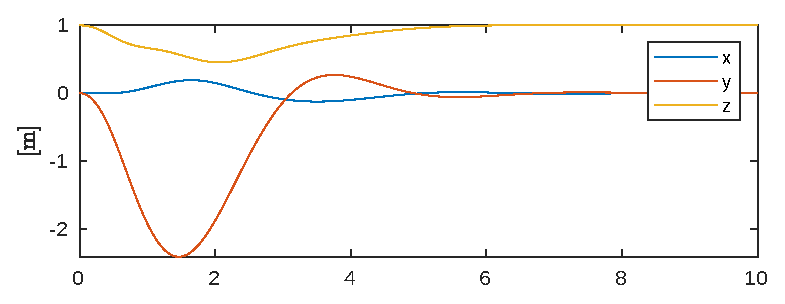
\includegraphics[width=0.8\linewidth]{fig/pos_edf}
    \caption{Posición del vehículo}
    \label{fig:pos_edf}
\end{figure}

\begin{figure}[!ht]
    \centering
    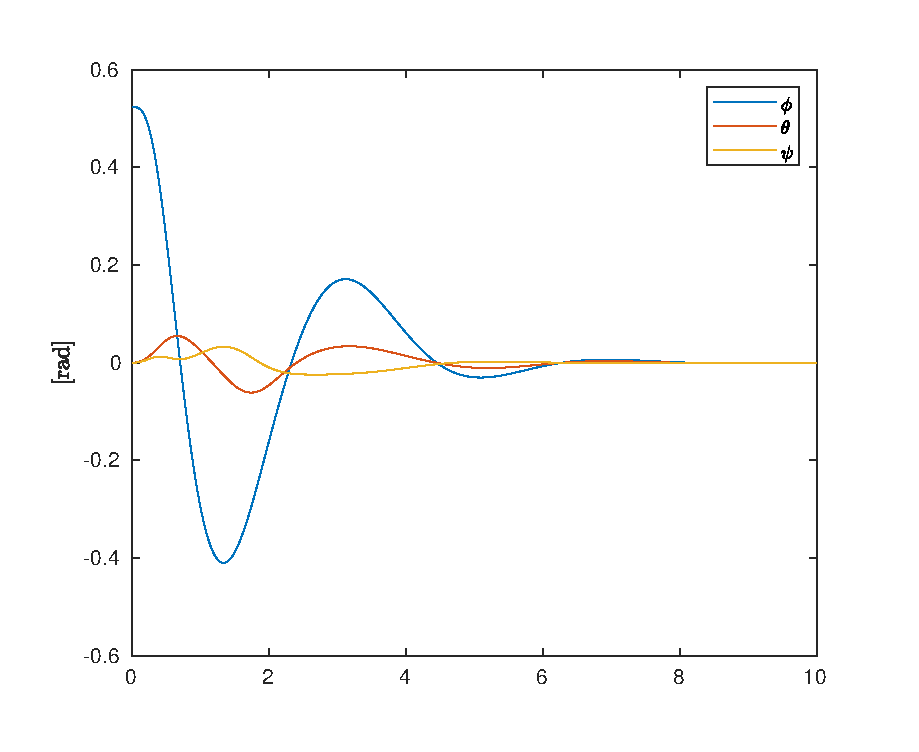
\includegraphics[width=0.6\linewidth]{fig/eulerang_edf}
    \caption{Ángulos de euler. Note que solo hubo perturbación inicial en $\phi$ sin embargo la actuación del gimbal ($\alpha$) generó una perturbación interna en $\theta$ por el efecto giroscópico.}
    \label{fig:eulerang_edf}
\end{figure}

\begin{figure}[!ht]
    \centering
    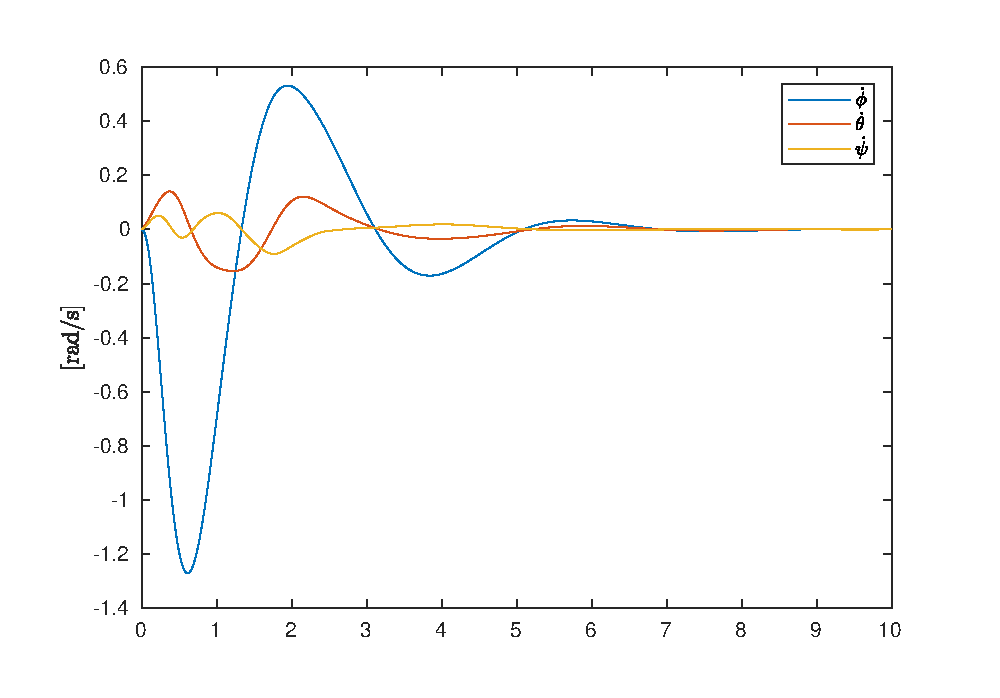
\includegraphics[width=0.6\linewidth]{fig/angvel_edf.eps}
    \caption{Velocidad angular del vehículo}
    \label{fig:angvel_edf.eps}
\end{figure}

\begin{figure}[!ht]
    \centering
    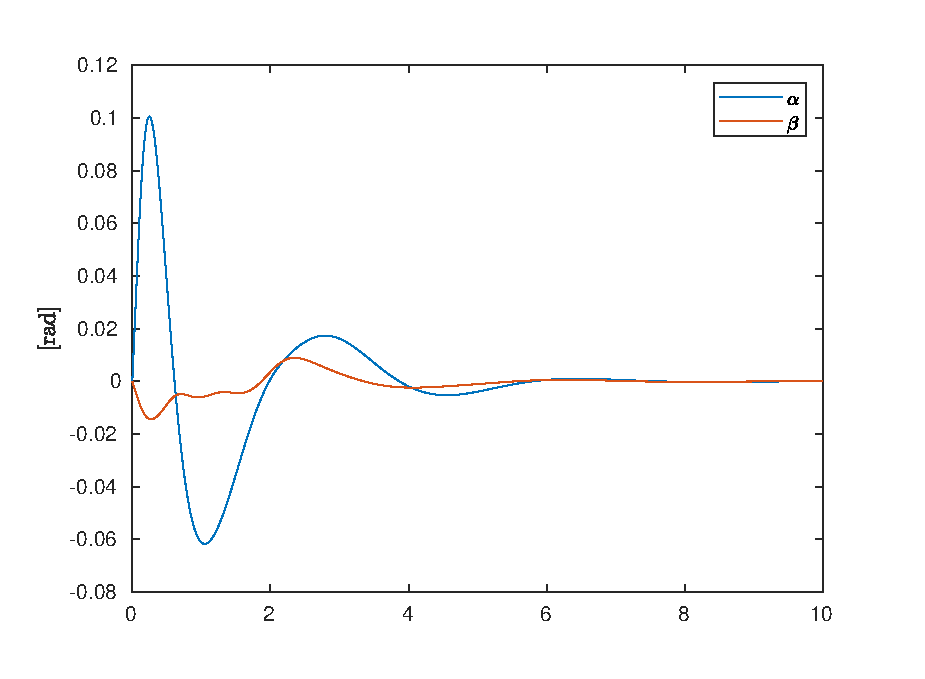
\includegraphics[width=0.6\linewidth]{fig/actuator_edf}
    \caption{Actuación angular del gimbal.}
    \label{fig:actuator_edf}
\end{figure}

\begin{figure}[!ht]
    \centering
    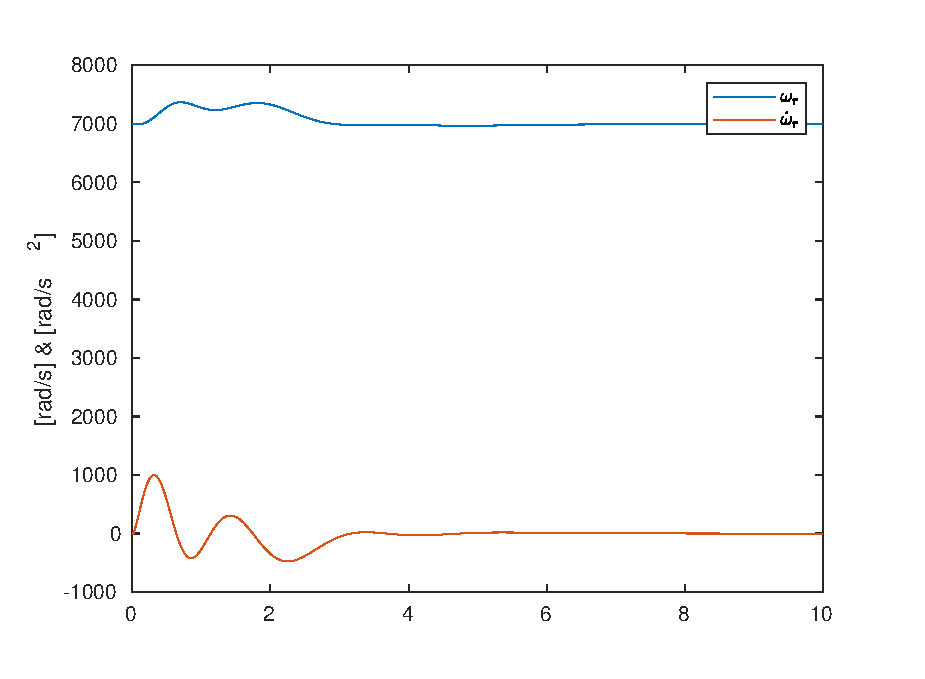
\includegraphics[width=0.6\linewidth]{fig/rotor_edf}
    \caption{Velocidad y aceleración angular del rotor.}
    \label{fig:rotor_edf}
\end{figure}





\section{Desarrollo de software}

\subsection{Introducción a Software Engineering}

Hay una rama de ingeniería conocida como \textit{Software Engineering}. Se dice que el nombre fue concebido por Margaret Hamilton, una renombrada ingeniera de la NASA quien fue la principal contribuidora al software de la misión Apolo 11 entre 1961 y 1969. El término entro en prominencia en 1968 en una conferencia de la OTAN en Alemania. En la conferencia se discutió la crisis del software, la cual se refiere a la dificultad de escribir software de calidad en el tiempo y presupuesto asignado. Este documento estaba adelantado a su tiempo y es considerado un clásico en la ingeniería de software \citep{natoSoftwareEngineering}.

\medskip

El documento de la OTAN fue escrito por personalidades renombradas de la ciencia de la computación como Edger Djikstra, Doug Mccllroy, y Alan Perlis. Unos de los temas centrales que se discute es la complejidad de programas como una fuente de problemas. A continuación se citan algunos fragmentos del documento traducidos:
\begin{quote}
    Particularmente alarmante es la falabilidad inevitable de programas grandes, ya que una una falla en un sistema hardware-software avanzado puede ser la diferencia entre la vida y la muerte.

    -- David and Fraser
\end{quote}

\begin{quote}
   Estoy preocupado por el crecimiento actual de los sistemas [...] ¿Deberíamos tener sistemas de este tamaño y complejidad?

    -- Opler
\end{quote}

Cualquier persona que haya emprendido a diseñar un sistema complejo entiende de donde vienen estos comentarios. Aún teniendo un entendimiento profundo del problema a resolver y de las herramientas a usar, \textit{el diseño nunca deja de ser un proceso iterativo} [Kinslow] en donde la \textit{simplicidad y claridad de la solución se vuelve un objetivo central y crucial.}


\subsection{Tecnologías usadas}

La decisión de software a utilizar dependió del controlador, poder de cálculo disponible, interfases de periféricos y funcionalidad deseada.

\medskip

Dado el uso de una Raspberry Pi,\footnote{La Raspberry Pi provee un entorno con Linux instalado que permite la programación con virtualmente cualquier lenguaje de programación en existencia.} el lenguaje de programación elegido fue \textbf{Go} (Golang) debido a los siguientes puntos

\begin{description}
    \item[Seguro] - Modelo de memoria Go, sistema de tipado fuerte\footnote{Hoy en día hay pocos lenguajes con sistemas de tipos fuertes. Contrario a la creencia popular, C y C++ ambos son tipados débilmente (se puede castear tipos implicitamente sin errores de compilador).}
    \item[Legible] - Claridad de sintaxis 
    \item[Simple] - Solo 80 carillas de especificación comparado a 1700 de ISO C++.
    \item[Concurrencia] - Crear \glsplural{corrutina} es simple, paralelizar corrutinas es trivial
    \item[Rendimiento] - Superior a Python, Java y Matlab. Comparable a C. Esto también implica un menor consumo de energía \citep{pythonIsSlow}.\footnote{El autor reconoce que este documento tiene sus defectos al momento de evaluar los lenguajes de programación ya que los programas provistos al \textit{Benchmarks Game} están condicionados a ciertas reglas artificiales que no son representativos de lo que son capaces los lenguajes. Dicho esto el comentario sobre el rendimiento es válido en la experiencia del autor en base a programas reales escritos en Python, Matlab y Go. Cabe destacar que si a algún lenguaje no fue evaluado de forma favorable en el paper de Pereira es Go ya que varias soluciones mucho más efectivas fueron propuestas por la comunidad de Go pero descartadas por los autores del \textit{Benchamrks Game} por no manejar la memoria igual que otros lenguajes.}
    \item[Estable] - \textit{The Go 1 promise} (La promesa Go 1)
    \item[Comprobado] -  Usado en sistemas de alto-riesgo/alta-complejidad (Kubernetes, Docker, Go-HEP)
    \item[Portable] - Todos los programas Go compilan a código nativo (código de máquina) para cualquier arquitectura y sistema operativo. Incluso se puede programar microcontroladores (TinyGo)
\end{description}

\subsection{Flujo de control}
\begin{figure}[!htb]
    \centering
    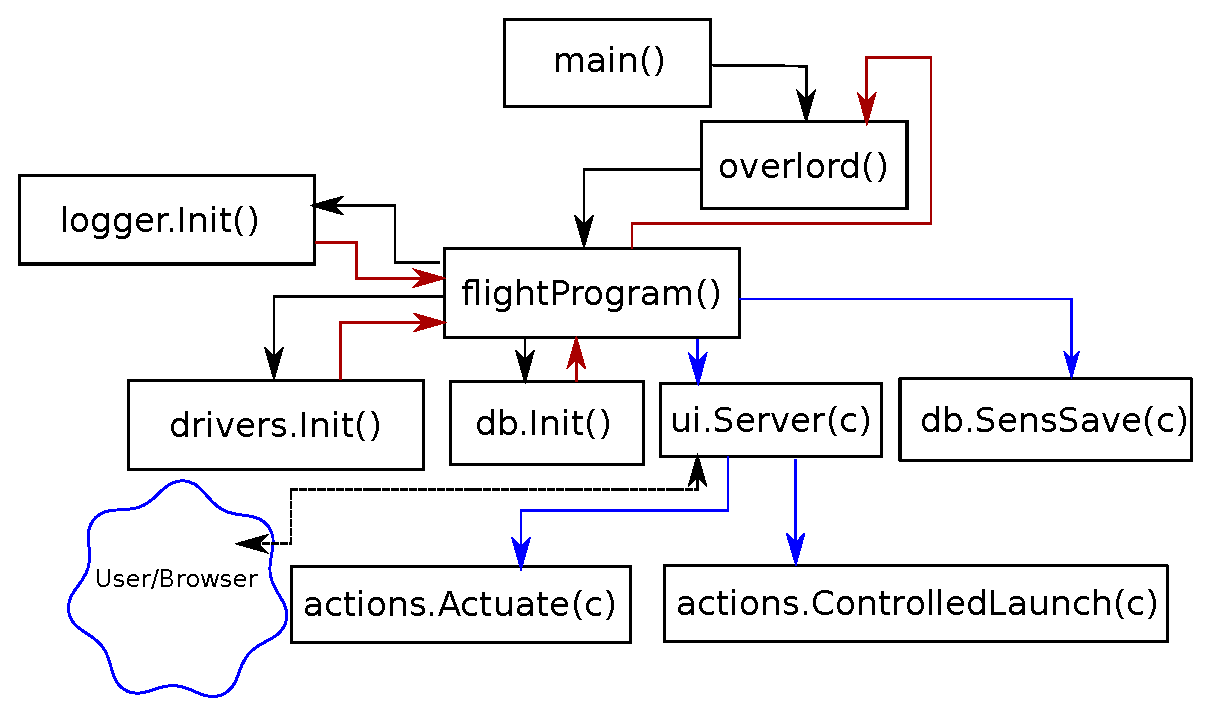
\includegraphics[width=0.7\textwidth]{fig/cfg_flightprogram.eps}
    \caption{Gráfico de flujo de control (CFG) del programa de vuelo. Las lineas de flujo azules son corrutinas independientes al programa principal. Las lineas negras son flujo del programa principal. Las lineas rojas son flujo del programa principal al encontrar un error.}
    \label{fig:flightProgram}
\end{figure}

Se ilustra el flujo de control a grandes rasgos usando un CFG en la figura \ref{fig:flightProgram}. El programa principal corrió la rutina \texttt{overlord} que a su vez comandó \texttt{flightProgram} y esperó que esta devuelva control a \texttt{overlord}. El propósito de \texttt{overlord} fue guardar el estado del vehículo y ante una falla irrecuperable en \texttt{flightProgram}, terminar con todas las corrutinas generadas por \texttt{flightProgram} y sus afiliadas y a su vez reiniciar \texttt{flightProgram} nuevamente con el último estado antes de la falla.


\subsection{Interfaz con hardware}

Como se mencionó anteriormente, la computadora elegida tiene varios puertos que sirviern como interfases con periféricos, entre ellos 

\begin{itemize}
    \item ADC (sensores)
    \item Generadores de PWM (para actuadores)
    \item Blinkenlights
\end{itemize}

Para la interacción del software con el hardware se usó la librería \href{https://periph.io}{periph.io}. Esta librería permitió la interacción a través de los puertos de comunicación de la Raspberry Pi. Los drivers para los periféricos fueron programados según la información dada en las datasheet.


\subsection{Implementación}

Los siguientes datos son provistos para dar una idea de la complejidad del programa y de las capacidades de la computadora usada.

Al momento de escribir el presente informe el programa de vuelo tuvo 3540 líneas de lógica, de las cuales 1680 correspondieron a los drivers de control de periféricos.

Se logró controlar la actuación de hasta 12 señales PWM y en simultaneo leer 16 señales de telemetría y guardar a archivo en una tarjeta SD a 1200 muestras por segundo (cada canal). 1060 líneas de código fueron dedicadas a la interfaz de usuario para facilitar el control del vehículo desde un browser, como por ejemplo Firefox.

\subsection{Debugging}

En junio 2021 se halló un bug en el software. Al cabo de cierto tiempo entraba en un estado degenerado el sistema donde no respondía a inputs de usuario ni a señales del sistema operativo. Debido a los periféricos usados la última señal transmitida al actuador se quedaba fija y era imposible retornar el sistema a un estado seguro sin terminar el programa forzosamente y reiniciarlo. 

Se sospechaba que el bug era causa de una falla en el kernel de Linux para computadoras ARM o corrupción de memoria causada por el garbage collector de Go. Debido a la configuración de la computadora y las herramientas disponibles para Go era dificil debuggear. El debugger nativo de Go (Delve) no funcionaba aún en procesadores ARM de 32 bits y el detector de carreras de Go tampoco estaba disponible para procesadores ARM. Se pasó 6 meses investigando intermitentemente y hablando con expertos en software y hardware.

En enero 2022 se encontró el mismo comportamiento observado durante el bug mientras se desarrollaba un proyecto no asociado a este trabajo. En este software el estado degenerado era causado por una condición de carrera, específicamente era el caso de una \gls{datarace}. Con este conocimiento se modificó el programa de vuelo para que pueda correr en un entorno de computadora desktop. Para lograr esto se programó un mock de la escritura I2C que fue facilitado por el uso de \textit{interfaces} en Go. Esta modificación permitió al detector de carreras de Go encontrar condiciones de carrera en el programa de vuelo. Se encontraron y se arreglaron 2 condiciones de carreras causadas por error de programador debido al uso equivocado de mutexes.

Aún así el error persistía y el programa seguía encontrandosé en el estado degenerado. Se optó por reescribir el programa y aplicando patrones de diseño más estrictos y seguros en base a lo aprendido en el primer intento. Al cabo de un mes se había reescrito el programa de vuelo de la empresa y el bug no volvió a resurgir en el desarollo. Esto se puede deber a que se redujo el uso de librerias de terceros y la cantidad de líneas de código totales bajó de 700.000 a tan solo 30.000, incluyendo dependencias de terceros. Excluyendo las liberías de terceros, la base de código era de tan solo 2100 líneas e incluía el frontend (interfaz con el usuario). Esta reducción de lineas de código logró una reducción de complejidad enorme a la base de código y permitió que el programa de vuelo sea más fácil de debuggear y mantener, lo cual fue beneficioso para los programadores e incluso para la empresa ya que el programa sería mantenido por otros programadores en el futuro.




\subsection*{Agradecimientos}
Dan Etenberg por hacer todo posible. Ben Romarowski por ayuda con la dinámica de cuerpo rígido y aerodinámica de los álabes.




\bibliography{tex/biblio} % Indica archivo
\bibliographystyle{plainnat} %estilo de bibliografía
% \bibliographystyle{unsrtnat}
%\includepdf[fitpaper=false,landscape]{pdf/Vistaexplotada5.pdf}
\end{document}
